% # Suggested Steps
% Find some data for experiments. You can use all films with titles, directors, actors and other related information. Some other data such as 'Infected cases by COVID-19', 'Stock data', 'Library data' etc. is also fine. But the size should be reasonably large.
% Store the data into a database table. Then use select in SQL to find the films with word "XXX" in titles, and record the execution time.
% Store the data into a file, and then load it into RAM. The data in RAM can be any format you preferred. Design an algorithm to search "XXX" in titles. Record the execution time of your algorithm.
% Some other comparisons and experiments you would like to do. Such as you can reorganize data into some other format for faster retrieval. You are recommended to study the mechanism of DMBS for storing and retrieval
%
% # Basic Requirements
% 1. Clearly and easy understanding design.
% 2. You need to show that you really do the experiments by some experimental details and reasonable analysis.
%
% # Bonus
% 1. High concurrency and transaction management
% 2. User privileges management
% 3. Database index and file IO
% 4. Large data sets (the data is large enough and cannot be stored into RAM)
% 5. Compare performance of multiple databases with file system over different operation systems
%
% # References
% 1. https://stackoverflow.com/questions/4279358/pythons-underlying-hash-data-structure-for-dictionaries
\title{通过 \bilibili\ 数据集探究数据库管理系统的性能优势}

\maketitle\tableofcontents\clearpage

\section{介绍}
本实验的目的是通过 \bilibili\ 数据集探究自己实现的数据库部分功能与 \texttt{DBMS} 之间的性能差异,同时比较不同 \texttt{DBMS} 之间的区别,最后利用 \texttt{DBMS} 提高数据的检索能力,加速数据分析。



\section{实验设计}
\subsection{实验数据和环境}
原先数据集爬取 \bilibili\ 知名或有争议的 UP 主(具体见附录~\ref{A:config})全部视频下的全部评论,用以做水军等检测,因此数据库课程的 Project 可以拿来直接使用。
但是个人觉得数据集不够完整,因此在数据库建模部分增加用户及视频表格,并通过外键将三张表关联起来。
前期下载数据量有些大,用户数量约五百万,如果将全部用户信息爬下来时间较长,因此放弃。
同时期间有被永久封禁的用户,现在已经找不到其个人信息,所以数据库建模时用户信息省略,仅保存其 uid。
当然为了以后研究方便,并未取消用户表格,所以数据库中共有三张表格:\verbbox{User}、\verbbox{Video}、\verbbox{Comment}。
数据库建模可视化如图~\ref{F:workbench-model},同时利用数据库对象关系映射\cite{sqlalchemy2020sqlalchemy}进行数据库建模,但是为进行跨文件系统的查询,因此有不符合范式的地方,数据库采用 \texttt{PostgreSQL}、\texttt{MySQL} 与 \texttt{SQLite},操作系统采用 \texttt{Linux},具体代码见附录~\ref{A:database}。

\begin{figure}[H]
    \centering
    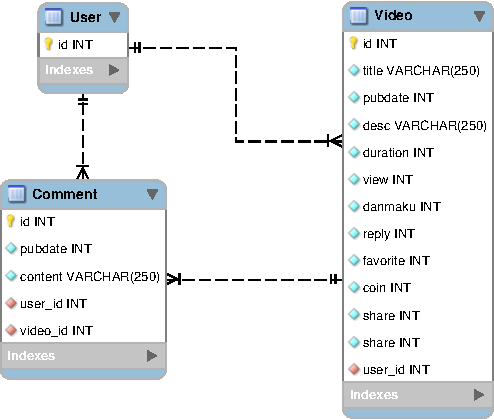
\includegraphics[width=.5\textwidth]{figures/1.pdf}
    \caption{Workbench 数据库模型}\label{F:workbench-model}
\end{figure}

所有数据分为三个文件夹,分别存储用户信息、视频信息以及评论信息,用户信息文件夹仅保存 UP 主的信息及出现在评论区全部用户的 uid,例如:
\begin{python}{users/546195.json}
{"name": "老番茄", "sex": "男", "face": "http://i2.hdslb.com/bfs/face/bc5ca101313d4db223c395d64779e76eb3482d60.jpg", "sign": "新浪微博:_老番茄_", "level": 6, "birthday": "08-13", "archive_view": 909097528, "article_view": 0, "likes": 37261387, "following": 1, "follower": 9548766}
\end{python}
视频信息文件夹保存全部视频的信息,例如:
\begin{python}{videos/av84887919.json}
{"pic": "http://i2.hdslb.com/bfs/archive/202bc40ecf4991d21df91f52a2d112eddb977de1.jpg", "title": "最强自夸王!!!!!", "pubdate": 1579924812, "desc": "歌曲:《自夸小队》\n作词/演唱:某幻君,老番茄,中国boy超级大猩猩,花少北\nHOOK:茶理理理子\n编曲:Lglywww \n混音:Blue coat\n摄影:藤井旋风,大饼\n后期:藤井旋风", "duration": 231, "owner": 1577804, "view": 11436611, "danmaku": 224768, "reply": 26880, "favorite": 530197, "coin": 989930, "share": 130342, "like": 956804}
\end{python}
评论信息文件夹按照视频通过嵌套字典保存保存全部评论信息,第一层的键为用户的 uid,第二册的键为时间戳,第二层的值为评论内容,后期更新代码可以保存评论的全部信息,但是本次 Project 仅考虑用户及时间戳,例如:
\begin{python}{comments/av3051327.json}
{"585481": {"1444662778": "作为天天刷太平洋的刷子团,今天在运送车队这个准备任务上载跟头了,来看看妹子的抢劫放松一下"}, "10917828": {"1444665830": "这期有点恶意卖萌    不过还好  反正我看了"}, "8872386": {"1444671846": "么么哒(`・ω・´)"}, "342211686": {"1581531133": "考古[呲牙][呲牙]"}, "29407696": {"1530278286": "考古"}, "3999038": {"1444689968": "来顶(づ ●─● )づ"}, "7266479": {"1444661483": "44444444先投币点赞在说"}, "495569": {"1444661357": "第三(`・ω・´)"}, "5713034": {"1444659325": "第二^_^"}, "2812699": {"1444658015": "第一(⌒▽⌒)"}, "6306456": {"1497997152": "╮( ̄▽ ̄)╭"}, "15514305": {"1493999905": "考古(=・ω・=)感觉每天就指紫雨视频活了"}, "10954013": {"1547426274": "๑乛◡乛๑"}, "74234761": {"1535518362": "考古"}}
\end{python}

数据库中的用户表格共有 5890919 行数据,视频表格共有 24742 行数据表格,评论共有 34097426 行数据,纯文本数据共有 3.7 G。
全部的程序见 \href{https://github.com/Iydon/homework/tree/master/CS307}{GitHub},至于 \bilibili\ 工具类例如兼容 bv 索引的爬虫见 \href{https://github.com/iydon/bilibili}{GitHub},预计 2020 年 4 月 1 日开源。代码使用 \texttt{Python} 语言,通过 \texttt{pipenv} 进行虚拟环境管理,具体见附录~\ref{A:config}。


\subsection{实验细节}
时间记录均为多次实验(5 次),后对时间取平均值,减少误差。

首先进行比较 \texttt{DBMS} 与 \texttt{RAM},根据 \texttt{Python} 中 Hashmap 的设计\cite{python2010rees}以及实际的计算,发现 \verbbox{Video} 表格可以导入内存,在硬盘中因为由许多小文件,所以大小为 98M。
\texttt{Python} 中因为涉及到指针,使用 \texttt{sys.getsizeof} 计算对象大小会造成误差,因此通过递归方式对原对象解构,得出内存中数据大小为 22M,同时以 \verbbox{Video.id} 为数据库索引。实验将 IO 读取与 \texttt{RAM} 索引进行分别计时,但是由于爬取的数据为 Json 格式,解析耗时较长,因此预处理为 CSV 格式,同时实现序列化 CSV 格式文件的功能(堵塞方式读取),提升效果显著。
其中 SQL 语句为 \texttt{select * from Video as v where v.title like "\%substr\%"},其中 \texttt{substr} 可以为任意关键词,本次实验选取 \bilibili\ 标题中较容易火的关键词:“震惊”、“内幕”、“锤”、“抑郁”、“盗”、“赞”。
最后结果如图~\ref{F:dbms_vs_ram}。

接下来进行不同 \texttt{DBMS} 之间的比较,包括 \texttt{PostgreSQL}、\texttt{MySQL} 与 \texttt{SQLite}。因为采用 \texttt{ORM} 进行数据库建模,因此在不同数据库之间转换较为容易,可以通过程序进行比较而非手动运行并记录数据。本次实验选取了五个方面:检索小数据库(\verbbox{Video})、检索大数据库(\verbbox{Comment})、使用关联对象、聚合函数以及分组。
最后结果如图~\ref{F:different_dbms}。

最后的实验则测试实现相同功能的 \texttt{Python} 程序与 \texttt{DBMS} 之间的区别,具体可以见第~\ref{S:extra} 节,因为前些天电脑出问题重装,原先程序丢失,所以并无对比,但是直观可以感受到 \texttt{DBMS} 的效率要远高于相同功能的程序,且不需要进行复杂的逻辑判断,只需要构造相应的 \texttt{SQL} 语句即可。


\subsection{实验结果}
第一次实验虽然 \texttt{DBMS} 性能略差于直接使用 \texttt{RAM} 读取数据,但是它们之间进行比较是不公平的,因为 \texttt{DBMS} 每次得到请求会通过硬盘索引数据,所以 \texttt{RAM} 读取数据的结果应加上 IO 消耗的时间,同时考虑到自己的程序只对单个 CSV 格式文件进行解析序列化,如果增加复杂的关系等,拓展性是不如 \texttt{DBMS},因此 \texttt{DBMS} 更为出色。
\begin{figure}[H]
    \centering
    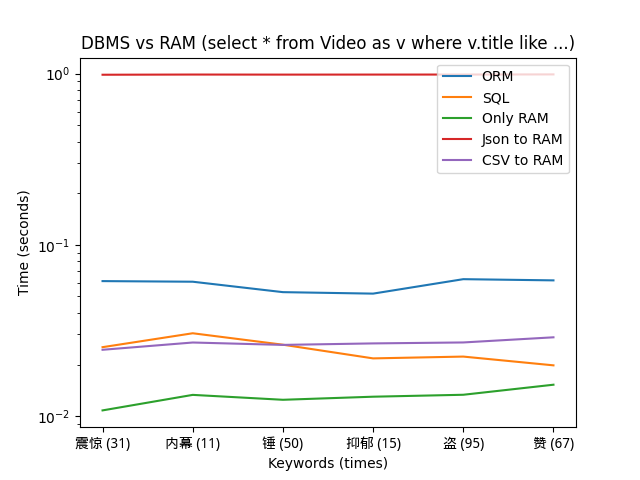
\includegraphics[width=.5\textwidth]{code/plot/dbms_vs_ram.png}
    \caption{\texttt{DBMS} 与 \texttt{RAM} 比较}\label{F:dbms_vs_ram}
\end{figure}

第二次实验在 98M 与 3.4G 的数据量上可以看出大概的趋势,即 \texttt{PostgreSQL} 较优于 \texttt{SQLite} 较优于 \texttt{MySQL}。这个结果有些不符合直觉,因为 \texttt{SQLite} 将所有数据保存为一个文件,同时本次实验只进行索引,可能这个数据量小于 \texttt{MySQL} 的优势区间。但是 \texttt{SQLite} 的劣势显而易见:缺乏用户管理与性能优化的灵活性。
\begin{figure}[H]
    \centering
    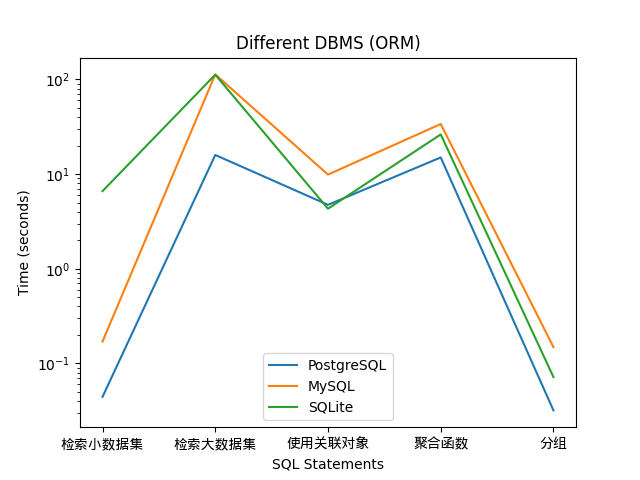
\includegraphics[width=.5\textwidth]{code/plot/different_dbms.png}
    \caption{不同 \texttt{DBMS} 比较}\label{F:different_dbms}
\end{figure}



\section{结论}
使用 \texttt{DBMS} 对持久化数据进行管理有非常大的优势,不仅其管理数据速度快,而且其响应时间较小。同时 \texttt{DBMS}(除报告中使用的 \texttt{SQLite})可以通过事务管理对用户数据进行保护,避免低权用户操作敏感数据。同时参考相应的文献可以得到 \texttt{DBMS} 的其他优势,例如并发能力、降低数据冗余、事务管理(Transaction Management)等。



\section{附加内容}\label{S:extra}
\subsection{提及到的 Bonus}
\begin{enumerate}
    \item 用户权限管理的思路是通过监控服务器某一端口(例如 42926),通过异步 IO 与高并发的方式,将不同用户的请求分为不同的协程,验证由安全散列算法生成的密码散列确定其权限,由服务器判断是否将数据返回给用户;
    \item 本实验的数据集约为 3.7G,其中 \verbbox{Comment} 约为 3.4G,前面的实验通过检索大数据集比较不同 \texttt{DBMS} 性能差异时使用了不能完全载入内存的数据。
\end{enumerate}


\subsection{提高检索能力,加速数据分析}
由于报告作者最近兼职在 \bilibili\ 做 \texttt{UP} 主,因此经常对其进行相应的数据分析,通过 \texttt{DBMS} 可以快速获取不同视频的点赞、投币、收藏的数据,并对其进行分析,如图~\ref{F:like-coin-favorite} 与图~\ref{F:like-coin-favorite-2}。
初步得出以下结论:
\begin{enumerate}
    \item 大概 2017 年之前点赞等更“值钱”一些(这里的”值钱“指的是当时大家看重推荐视频的权利,或者是有些数据丢失了造成了我的错觉,前者可能的解释是当时部分 UP 主是课余兴趣才投稿的,随着用户基数增大变成盈利手段,号召一键三连,这句话没有负面意思毕竟人是要吃饭的);
    \item 现在的部分知名 UP 主也是从早期粉丝少通过不断更新积累粉丝(发现知名 UP 主部分远古稿件的点赞等数据不好看,而且大部分人为考古,比如 老番茄、中国BOY 等,与现在有些“UP”短期粉丝快速增长活跃度低形成对比,这句话也没有负面意思毕竟有名气了到哪里粉丝都会关注);
    \item     不适当的评论或多来自于三观容易受影响的未成年人(简单看了公开资料,部分“不适当”的评论或来自于未成年人,当然可能也包括心智未成熟的部分成年人,部分 UP 主可能也没有注意到自己的视频中或多或少出现具有误导性、带“情感色彩”词汇,然后由观看者进行进一步加工,理解成为自己想要的意思,进而产生不适当言论,毕竟刷视频多了,分配到一个视频的思考时间与能力会相应减少,而且视频相较文本信息更容易接受)。
\end{enumerate}

\begin{figure}[H]
    \centering
    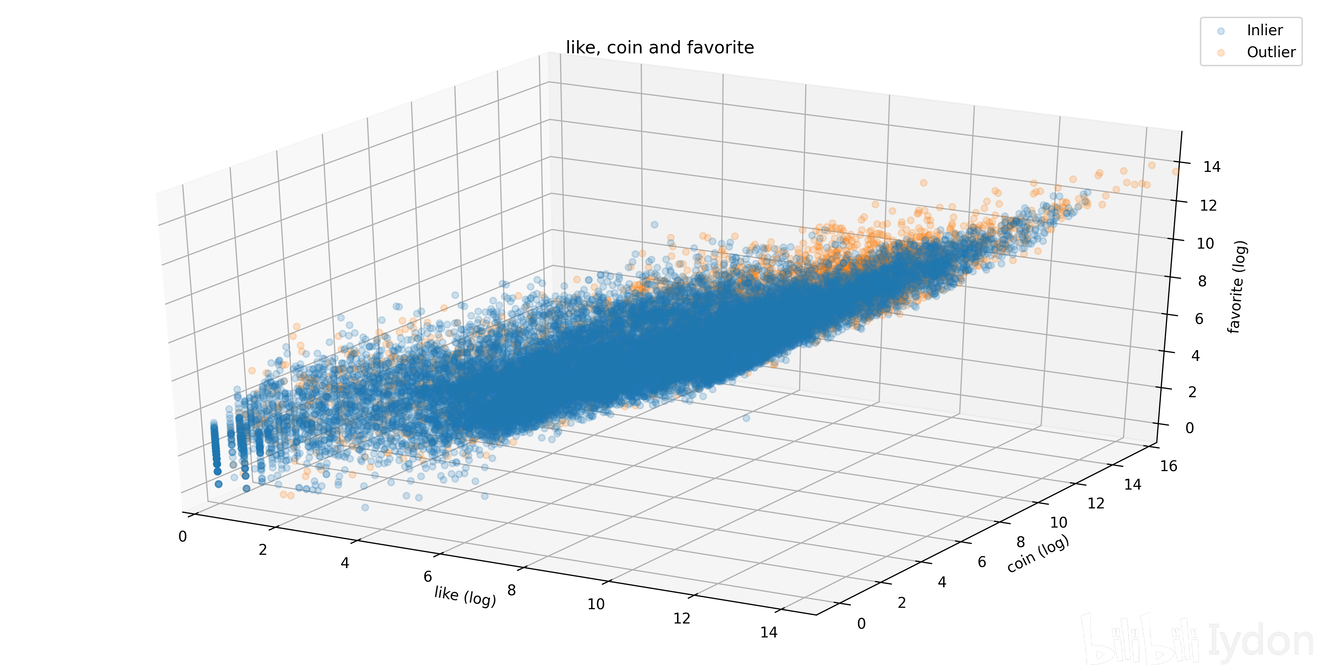
\includegraphics[width=.7\textwidth]{figures/like_coin_favorite.png}
    \caption{点赞 + 投币 + 收藏 直观展示图及离群值}\label{F:like-coin-favorite}
\end{figure}

\begin{figure}[H]
    \centering
    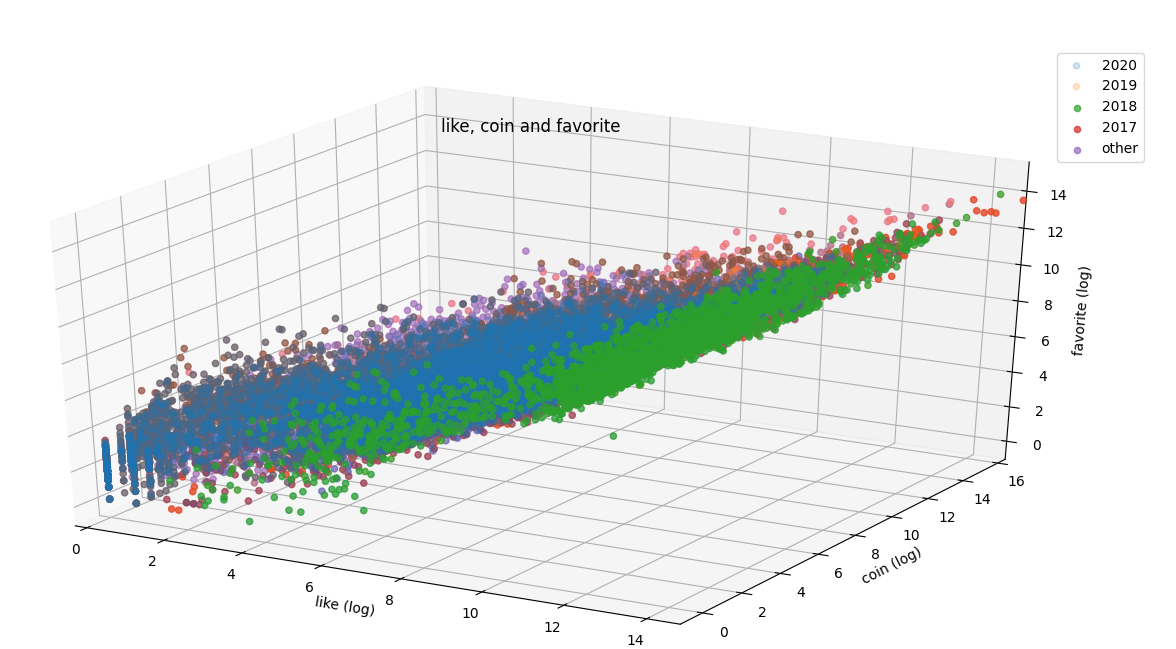
\includegraphics[width=.7\textwidth]{figures/like_coin_favorite-2.png}
    \caption{不同年份 点赞 + 投币 + 收藏 直观展示图}\label{F:like-coin-favorite-2}
\end{figure}

同时最近也尝试做更进一步的研究,敬请期待,详情请参考 \href{https://github.com/iydon/bilibili}{GitHub}。



\clearpage
\section{参考文献}
\nocite{*}
\printbibliography[heading=none]



\clearpage
\begin{appendices}
    \section{配置文件}\label{A:config}
        \pythonfile{../Pipfile}{Pipfile}
        \pythonfile{code/config.py}{config.py}
    \section{数据库建模}\label{A:database}
        \pythonfile{code/database.py}{database.py}
\end{appendices}
